\documentclass[runningheads]{llncs} % template "Lecture notes for computer science"
\usepackage[spanish]{babel} % para el texto en espanhol
\usepackage{graphicx} % para incluir imagenes, graficos, etc.
\graphicspath{{images/}} % ruta a la carpeta de imagenes
\usepackage{hyperref} % para los hipervinculos
\usepackage{xurl} % para el line breaker de los url
\usepackage{xcolor} % para definir colores custom
\hypersetup{ % configuracion de los hiper vinculos
    colorlinks=true,
    linkcolor=black,
    filecolor=black,      
    urlcolor=blue,
    citecolor=black, % ver si poner en blue o dejar asi
    pdftitle={Redes neuronales},
    pdfpagemode=FullScreen,
}
\usepackage[T1]{fontenc} % para la codificacion de la fuente.
\usepackage[backend=biber,style=numeric]{biblatex} % para la bibliografia.
\addbibresource{bibliografia.bib} % incluir el .bib
\setcounter{biburlnumpenalty}{9000} % Para el line breaker en URL con numeros (que tambien afecta a la bibliografia)
\setcounter{biburllcpenalty}{9000} % Para el line breaker en URL con letras minuculas (que tambien afecta a la bibliografia)
\setcounter{biburlucpenalty}{9000} % Para el line breaker en URL con letras mayusculas (que tambien afecta a la bibliografia)
\usepackage{csquotes} % para que los textos citados esten con tipografia de acuerdo con las reglas de csquotes
\usepackage{amsmath}

\begin{document}

% =================================================================================
% PORTADA
% =================================================================================
\title{Redes neuronales y sus aplicaciones recientes}

\author{Alain Vega\orcidID{Y11159} \\ \email{alainjosevz@gmail.com}}

\authorrunning{Alain Vega}

\institute{Universidad Catolica "Nuestra señora de la Asuncion" \\ 
Facultad de ciencias y tecnologia \\
Departamento de electronica e informatica \\
\url{https://www.universidadcatolica.edu.py/} }

\maketitle           

\begin{abstract}
Una de las tendencias ultimamente son las redes neuronales. En este documento
se muestran conceptos claves sobre este modelo y una significativa variedad
de ejemplos sobre aplicaciones recientes del mismo.

\keywords{Redes neuronales \and Inteligencia artificial \and Machine learning
\and Deep learning \and AI \and ML \and NN \and ANN \and SNN \and RNN 
\and CNN \and GAN \and DL}
\end{abstract}
% =================================================================================
% CONTENIDO
% =================================================================================
\section{Introduccion}
Si hace unos años, nos hubieran dicho que una máquina sería capaz de aprender 
por sí sola y tomar decisiones basadas en esa experiencia, ¿te lo habrías creído? 
¿Y si además te hubieran dicho que un conjunto de algoritmos serían capaces de
hacer funciones consideradas \textquotedblleft{humanas}\textquotedblright{}
como crear arte o componer melodías únicas? \cite{int1}

Todo esto es ya una realidad, por ello ultimamente la Inteligencia artificial (AI) 
esta en boca de todos, pero es gracias a las \textbf{redes neuronales} (NN)
que todo esto es posible. 

Estas redes alcanzan metas bastante impresionantes y que cada vez se acercan 
más a esa idea original de reproducir el funcionamiento del cerebro humano 
en una computadora. 

Ahora bien, ¿en qué consisten estos modelos? ¿Cómo puede imitar un computadora 
el proceso de aprendizaje y acabar desarrollando una
\textquotedblleft{cosa}\textquotedblright{} que funciona? \cite{int2}
\section{¿Que es una red neuronal?}
Una red neuronal, tambien conocida como red neuronal artificial (ANN)
o red neuronal simulada (SNN), es un modelo de \textit{machine learning} (ML)
el cual constituye el eje de los algoritmos de \textit{deep learning} (DL) 

Su nombre y estructura se inspiran en el cerebro humano, 
e imitan la forma en la que las neuronas biológicas se señalan entre sí.

Las redes neuronales artificiales (ANN) están formadas por capas de nodos, 
que contienen una capa de entrada, una o varias capas ocultas y una capa de salida.
\cite{def-ibm1}

Donde cada nodo se conoce como una neurona artificial, esta se conecta a 
otra neurona (nodo) la capa hace referencia a conjunto de nodos (neuronas).

\begin{figure}
    \centering
    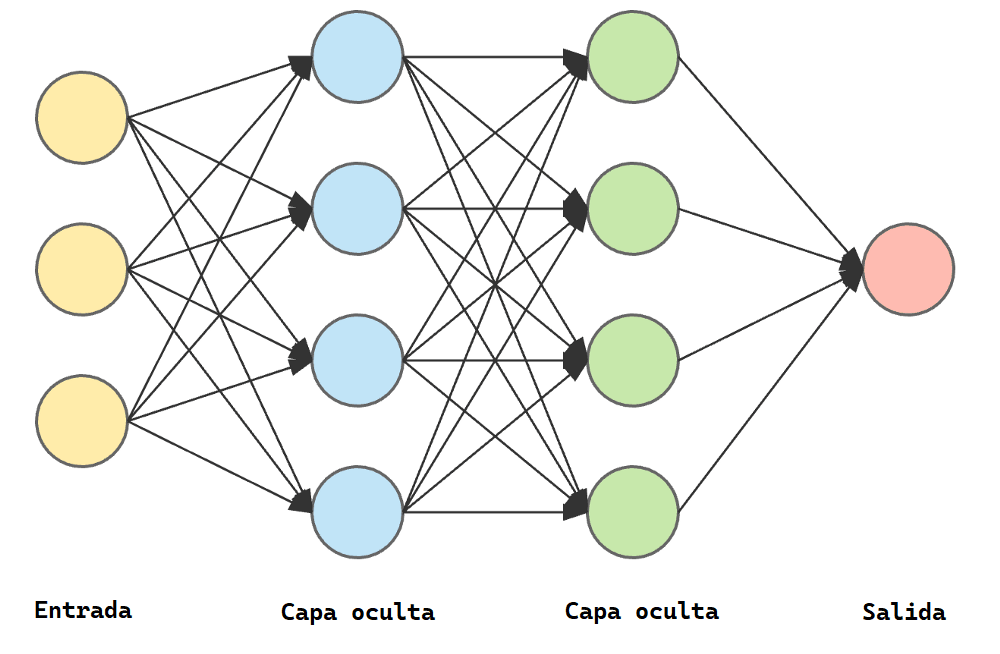
\includegraphics[scale=0.4]{red_neuronal_artificial.png}
    \caption{Ejemplo de una red neuronal artificial (ANN) \cite{int1}}
    \label{fig:red_neuronal_artificial}
\end{figure}

En la figura \ref{fig:red_neuronal_artificial} se muestra un ejemplo,
aqui la capa de la izquierda es la capa de entrada (la que esta
conectada con el \textquotedblleft{mundo}\textquotedblright{} exterior y se alimenta de el)
las capas 2 y 3 son capas ocultas que ayudan al procesamiento
de la tarea y por ultimo la capa 4 es la de salida, la cual
envia sus resultados al \textquotedblleft{mundo}\textquotedblright{} exterior

\section{Estructura basica de una red neuronal}
\subsection{Analogia con el cerebro}
La neurona es la unidad fundamental del sistema nervioso y en particular 
del cerebro. Cada neurona es una simple unidad procesadora que recibe y combina 
señales desde y hacia otras neuronas. 
Si la combinación de entradas es suficientemente fuerte la salida de la neurona
se activa. \cite{libro-def}

\begin{figure}
    \centering
    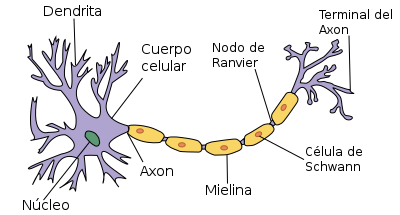
\includegraphics[scale=0.5]{neurona_real.png}
    \caption{Componentes de una reurona real \cite{img-neurona_real}}
    \label{fig:neurona_real}
\end{figure}

El cerebro consiste en uno o varios billones de neuronas densamente 
interconectadas. Apoyandonos en la figura \ref{fig:neurona_real}.
El axón (salida) de la neurona se ramifica y está conectada a las dendritas (entradas) 
de otras neuronas a través de uniones llamadas sinapsis.
La eficacia de la sinpasis es modificable durante el proceso de 
aprendizaje de la red. \cite{libro-def}

\subsection{Redes neuronales artificiales (ANN)}
En las Redes Neuronales Artificiales, ANN, la unidad análoga a la neurona biológica es
el elemento procesador, PE (\textit{Process Element}). Un elemento procesador tiene varias
entradas y las combina, normalmente con una suma básica. 
\footnote[1]{Existen mas formas de combinar las entradas de la neurona 
que la sumatoria, como por ejemplo con un productorio: \(\Pi_{i}{w_{i}*x_{i}}\)
o aplicando la funcion maximo elemento: \(\max_{i}{w_{i}*x_{i}}\) \cite{tesis-matich}}.
La suma de las entradas es
modificada por una función de transferencia y el valor de la salida de esta función de
transferencia se pasa directamente a la salida del elemento procesador.
\footnote[2]{En lugar de pasar el valor de la funcion de transferencia
directamente a la salida (funcion de salida = funcion identidad), 
se puede pasar por otra funcion, \textbf{la funcion de salida} 
la cual pueder ser una funcion binaria \cite{tesis-matich} \\
\(B(x)=1\) si \(x>=umbral\), \\
\(B(x)=0\) caso contario}

La salida del PE se puede conectar a las entradas de otras neuronas artificiales (PE)
mediante conexiones ponderadas correspondientes a la eficacia de la sinapsis de las
conexiones neuronales. \cite{libro-def}

\begin{figure}
    \centering
    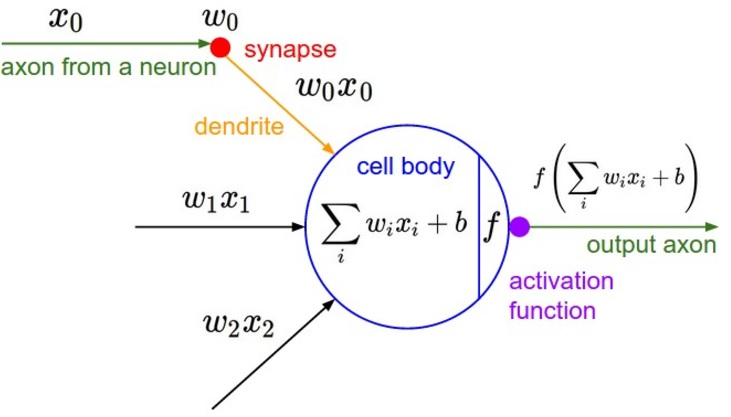
\includegraphics[scale=0.6]{neurona_artificial2.png}
    \caption{Diagrama de una neurona artificial con conceptos de una neurona real \cite{img-neurona_artificial2}}
    \label{fig:neurona_artificial}
\end{figure}

La Figura \ref{fig:neurona_artificial} muestra una neurona artificial con conceptos
de una neurona real.
La dendrita se representa como un enlace de entrada a la neurona.

La sinapsis se representa como la union/fusion de un terminal del axon de una neurona
con una dendrita de otra neurona. 

En el cuerpo celular ocurren varias cosas, la primera es que gracias a sinapsis las
entradas disponibles de cada una de las neuronas de la capa anterior llegan como el 
producto \(x_{i}*w_{i}\), donde \(x_{i}\) es el resultado de una neurona 
\textquotedblleft{anterior}\textquotedblright{} y \(w_{i}\) es el peso 
\textquotedblleft{conectarse}\textquotedblright{} a la dendrita de nuestra neurona.
La segunda es la sumatoria de cada entradas \(x_{i}*w_{i}\) y sumarle
\(b\) que representa el bias/sesgo/umbral (el cual nos permite mover la funcion
de activacion de manera horizontal).
Por ulitmo toda la sumatoria del paso dos, se pasa a la funcion de activacion \(f\)
esta puede lineal o no lineal, existen una amplia variedad de funciones de activacion.

Finalmente transmite el resultado \(y = f(\sum_{i=1}^{n}{x_{i}*w_{i}} + b)\)
suponiendo \textit{n} entradas

\section{Funcion de activacion}
La funcion de activacion se encarga de decidir cuando una neurona artificial debe activarse
o no. Esto significa que dicha funcion decide cuando la entrada a la neurona artificial
es importante o no para la red. \cite{fun-activacion}

Su rol es derivar la salida de la neurona artificial, dado un conjunto de valores de la entrada
para alimentar a otras neuronas artificiales. \cite{fun-activacion}

Existen muchas funciones de activacion, se pueden clasificar en tres grupos.
\subsection{Clases de funciones de activacion}

\subsubsection{Funciones de paso binario}
Necesita de un valor umbral \(\xi\) que decide cuando la neurona artificial debe activarse o no.
\cite{fun-activacion}

\[
    B(x) =
    \left \{
        \begin{aligned}
        0, \ \ & \text{si } x < \xi  \\
        1, \ \ & \text{si } x \geq \xi
        \end{aligned}
    \right .
\]

\subsubsection{Funciones de activacion lineales}
Tambien conocida como \textquotedblleft{}sin activacion\textquotedblright{} 
donde la activacion es proporcional a la entrada. \cite{fun-activacion2} \\
Se utilizan en la capa de salida para problemas de regresion lineal. \cite{fun-activacion}

\[ f(x)=mx+b \]

\subsubsection{Funciones de activacion no lineales}
Son las mas utilizadas ya que facilita que el modelo generice o se adapte con una 
variedad de datos y diferencie entre los resultados. \cite{fun-activacion2}

Las principales son: 
\begin{itemize}
    \item{\textbf{Sigmoide o logistica}: utlizada en la capa de salida
    para problemas de clasificacion binaria (clasificar en 2 grupos) y problemas
    de clasificacion multietiqueta o multi-objetivo (la salida puede estar 
    en mas de un grupo). \cite{fun-activacion}
    \[\sigma(x) = \frac{1}{1-e^{-x}}\] } 
    \item{\textbf{Tangente hiperbolico}: utilizada en las capas ocultas 
    de una red neuronal recurrent (RNN). \cite{fun-activacion}
    \[\tanh(x) = \frac{e^{x}-e^{-x}}{e^{x}+e^{-x}}\]}
    \item{\textbf{ReLU (\textit{Rectified Linear Unit})}: utilizada en las capas
    ocultas de una red neuronal convolucional (CNN). \cite{fun-activacion}
    \[ReLU(x) = max(0,x)\]} 
    \item{\textbf{Softmax}: utilizada en la capa de salida para problemas
    de multi-clasificacion (clasificar en mas de 2 grupos). \cite{fun-activacion}
    \[ s(x_{i}) = \frac{e^{x_{i}}}{\sum_{j=1}^{n}{e^{x_{j}}}} \]}\\
    La funcion Softmax convierte el vector de \textit{K} entradas a un vector 
    de \textit{K} salidas tal que la suma las salidas es igual a 1,
    entonces la salida se puede interpretar como una distribucion de probabilidades.
    \cite{fun-softmax}
\end{itemize}

\section{Conocimiento}
\subsection{¿Como aprenden estas redes?}
En el ciclio de vida de una ANN hay en general dos fases, las cuales son 
la fase de entrenamiento y la fase de pruebas. El proceso de determinar
los pesos y los sesgos (\textit{bias}) ocurren en la fase de entrenamiento. 
\cite{backpropagation}

Si el lector indaga sobre redes neuronales, encontrará dos términos esenciales 
que describen el movimiento de información a traves de la red 
\textbf{\textit{forward propagation}} y \textbf{\textit{back propagation}} \cite{fun-activacion}
de forma breve significan: 

\subsubsection{FowardPropagation:}
tambien conocida como \textit{forward pass} hace referencia al calculo y
almacenamiento de variables intermedias (incuyendo \textit{outputs}) para
una ANN para una ANN en orden desde la capa de entrada hasta la capa de salida. 
\cite{zhang2023dive}

\subsubsection{BackPropagation:}
se refiere al método de calcular el gradiente de los parámetros de la red neuronal. 
En resumen, el método atraviesa la red en orden inverso, desde la capa de salida a 
la de entrada, según la regla de la cadena del cálculo. 
El algoritmo almacena las variables intermedias (derivadas parciales) 
necesarias al calcular el gradiente con respecto a algunos parámetros.
\cite{zhang2023dive}

\subsubsection{Aprendizaje.}
Que una ANN \textquotedblleft{}aprenda\textquotedblright{} significa que
esta ajusta mejor sus parametros (pesos y sesgos).

Entonces, ¿cómo obtienen las redes neuronales valores óptimos de peso y sesgo? 
La respuesta es a través de un gradiente de error. \footnote[1]{Recientemente
se exploraron mas alternarivas debidos a problemas bien conocidos. \cite{alternativasBP}} 
Lo que queremos saber al fijar 
el peso y el sesgo actuales ¿necesitamos disminuir o aumentar nuestro valor actual?
es si los valores de peso y sesgo actuales son demasiado grandes o demasiado pequeños
(¿necesitamos disminuir o aumentar nuestro valor actual?) con respecto a su valor optimo? 
Y cuánto se desvía (¿ cuánto necesitamos disminuir o aumentar nuestro valor actual?) 
de sus valores óptimos. El gradiente que buscamos son las derivadas del error 
con respecto a ponderaciones y sesgos.\cite{backpropagation}

¿Porqué es eso? porque queremos saber cómo nuestros pesos y sesgos actuales afectan 
el valor del error de la red neuronal como referencia para responder 2 preguntas 
en el párrafo superior (disminuir o aumentar y cuánto). La forma en que obtenemos el valor 
del gradiente es a través de un algoritmo bien conocido llamado \textit{back propagation}. 
La forma en que utilizamos el gradiente que se obtuvo mediante \textit{back propagation} 
para mejorar el valor de peso y los sesgos es a través de un algoritmo de optimización.
\cite{backpropagation}

\subsection{¿Representa como aprendemos los humanos?}
Si bien las redes neuronales estan inspiradas en el cerebro humano, ¿esto significa 
que estas redes pueden verse como un cerebro humano simulado?, estudios recientes sugieren 
que podría no ser así. Un equipo del MIT examinó recientemente más de 11.000 redes neuronales 
y descubrió que sólo exhibían las características de procesamiento celular del pensamiento 
humano cuando estaban entrenadas para hacerlo. 

Sin esas restricciones, pocas redes desarrollaron la actividad similar a la de las células 
que puede usarse para predecir la funcionalidad cerebral real, que evoluciona naturalmente 
sin condiciones previas. \cite{NNvsANN}

\subsubsection{Diferencias de aprendizaje} 
Otra diferencia clave entre las redes neuronales y los cerebros vivos es la forma 
en que aprenden. Según Maxim Bazhenov, Ph.D. y profesor de medicina en la 
Facultad de Medicina de la Universidad de California en San Diego, 
las ANN sobrescriben datos antiguos a medida que se reciben nuevos datos mientras 
el cerebro se involucra en un aprendizaje continuo e incorpora nuevos datos para lograr 
mayores niveles de comprensión. \cite{NNvsANN}

\newpage
\section{Aplicaciones}
\subsection{ChatGPT}
Es una de las aplicaciones recientes mas reconocidas, ya casi no necesita presentacion
seguramente el lector ya conoce esta poderosa y util herramienta por expriencia propia.
Su exito fue tan grande que empresas como Google o Microsoft apresuraron sus proyectos
\textit{Bard} y \textit{Bing} respectivamente.

ChatGPT (\textit{Generative Pre-trained Transformer}) es un procesador del lenguaje natural
desarrollada por OpenAI, es un modelo hermano de InstructGPT, que esta capacitado
para seguir una instruccion en un mensaje y proporcionar una respuesta detallada.
\cite{ej-chatgpt}

El formato de diálogo hace posible que ChatGPT responda preguntas de seguimiento, 
admita sus errores, cuestione premisas incorrectas y rechace solicitudes inapropiadas.


\subsubsection{¿Como funciona?}
Se entrena el modelo utilizando \textit{Reinforcement Learning from Human Feedback}, 
(RLHF) es decir el aprendizaje por refuerzo a partir de la retroalimentacion humana,
similar a su hermano InstructGPT pero con ligeras diferencias en la configuracion de
recopilacion de datos. \cite{ej-chatgpt}

Se entrena un modelo inicial mediante ajustes supervisados: los entrenadores humanos
de la AI proporcionan conversaciones en las que juegan de ambos lados: el usuario
y un asistente de AI. Se les da a los capacitadores acceso a sugerencias escritas
por modelos para ayudarlos a redactar sus respuestas. 
Se mezcla este nuevo conjunto de datos de diálogo con el conjunto de datos de InstructGPT, 
el cual transforman en un formato de diálogo. \cite{ej-chatgpt}

Para crear un modelo de recompensa para el aprendizaje por refuerzo, 
se necesita recopilar datos comparativos, que consisten en dos o más respuestas 
del modelo clasificadas por calidad. Para recopilar estos datos, se toman conversaciones 
que los entrenadores de IA tuvieron con el chatbot. Seleccionan al azar un mensaje 
escrito por un modelo, prueban varias alternativas de finalización y se pide a los 
entrenadores de IA que las clasifiquen. Usando estos modelos de recompensa, 
ajustan el modelo usando la Optimización de Política Proximal (la cual es
una nueva clase de algoritmos de aprendizaje por refuerzo, que funcionan de manera
comparable o mejor que los enfoques actuales y, al mismo tiempo, son mucho mas
simples de implementar y ajustar \cite{def-PPO})

Realizan varias iteraciones de este proceso. \cite{ej-chatgpt}

\begin{figure}
    \centering
    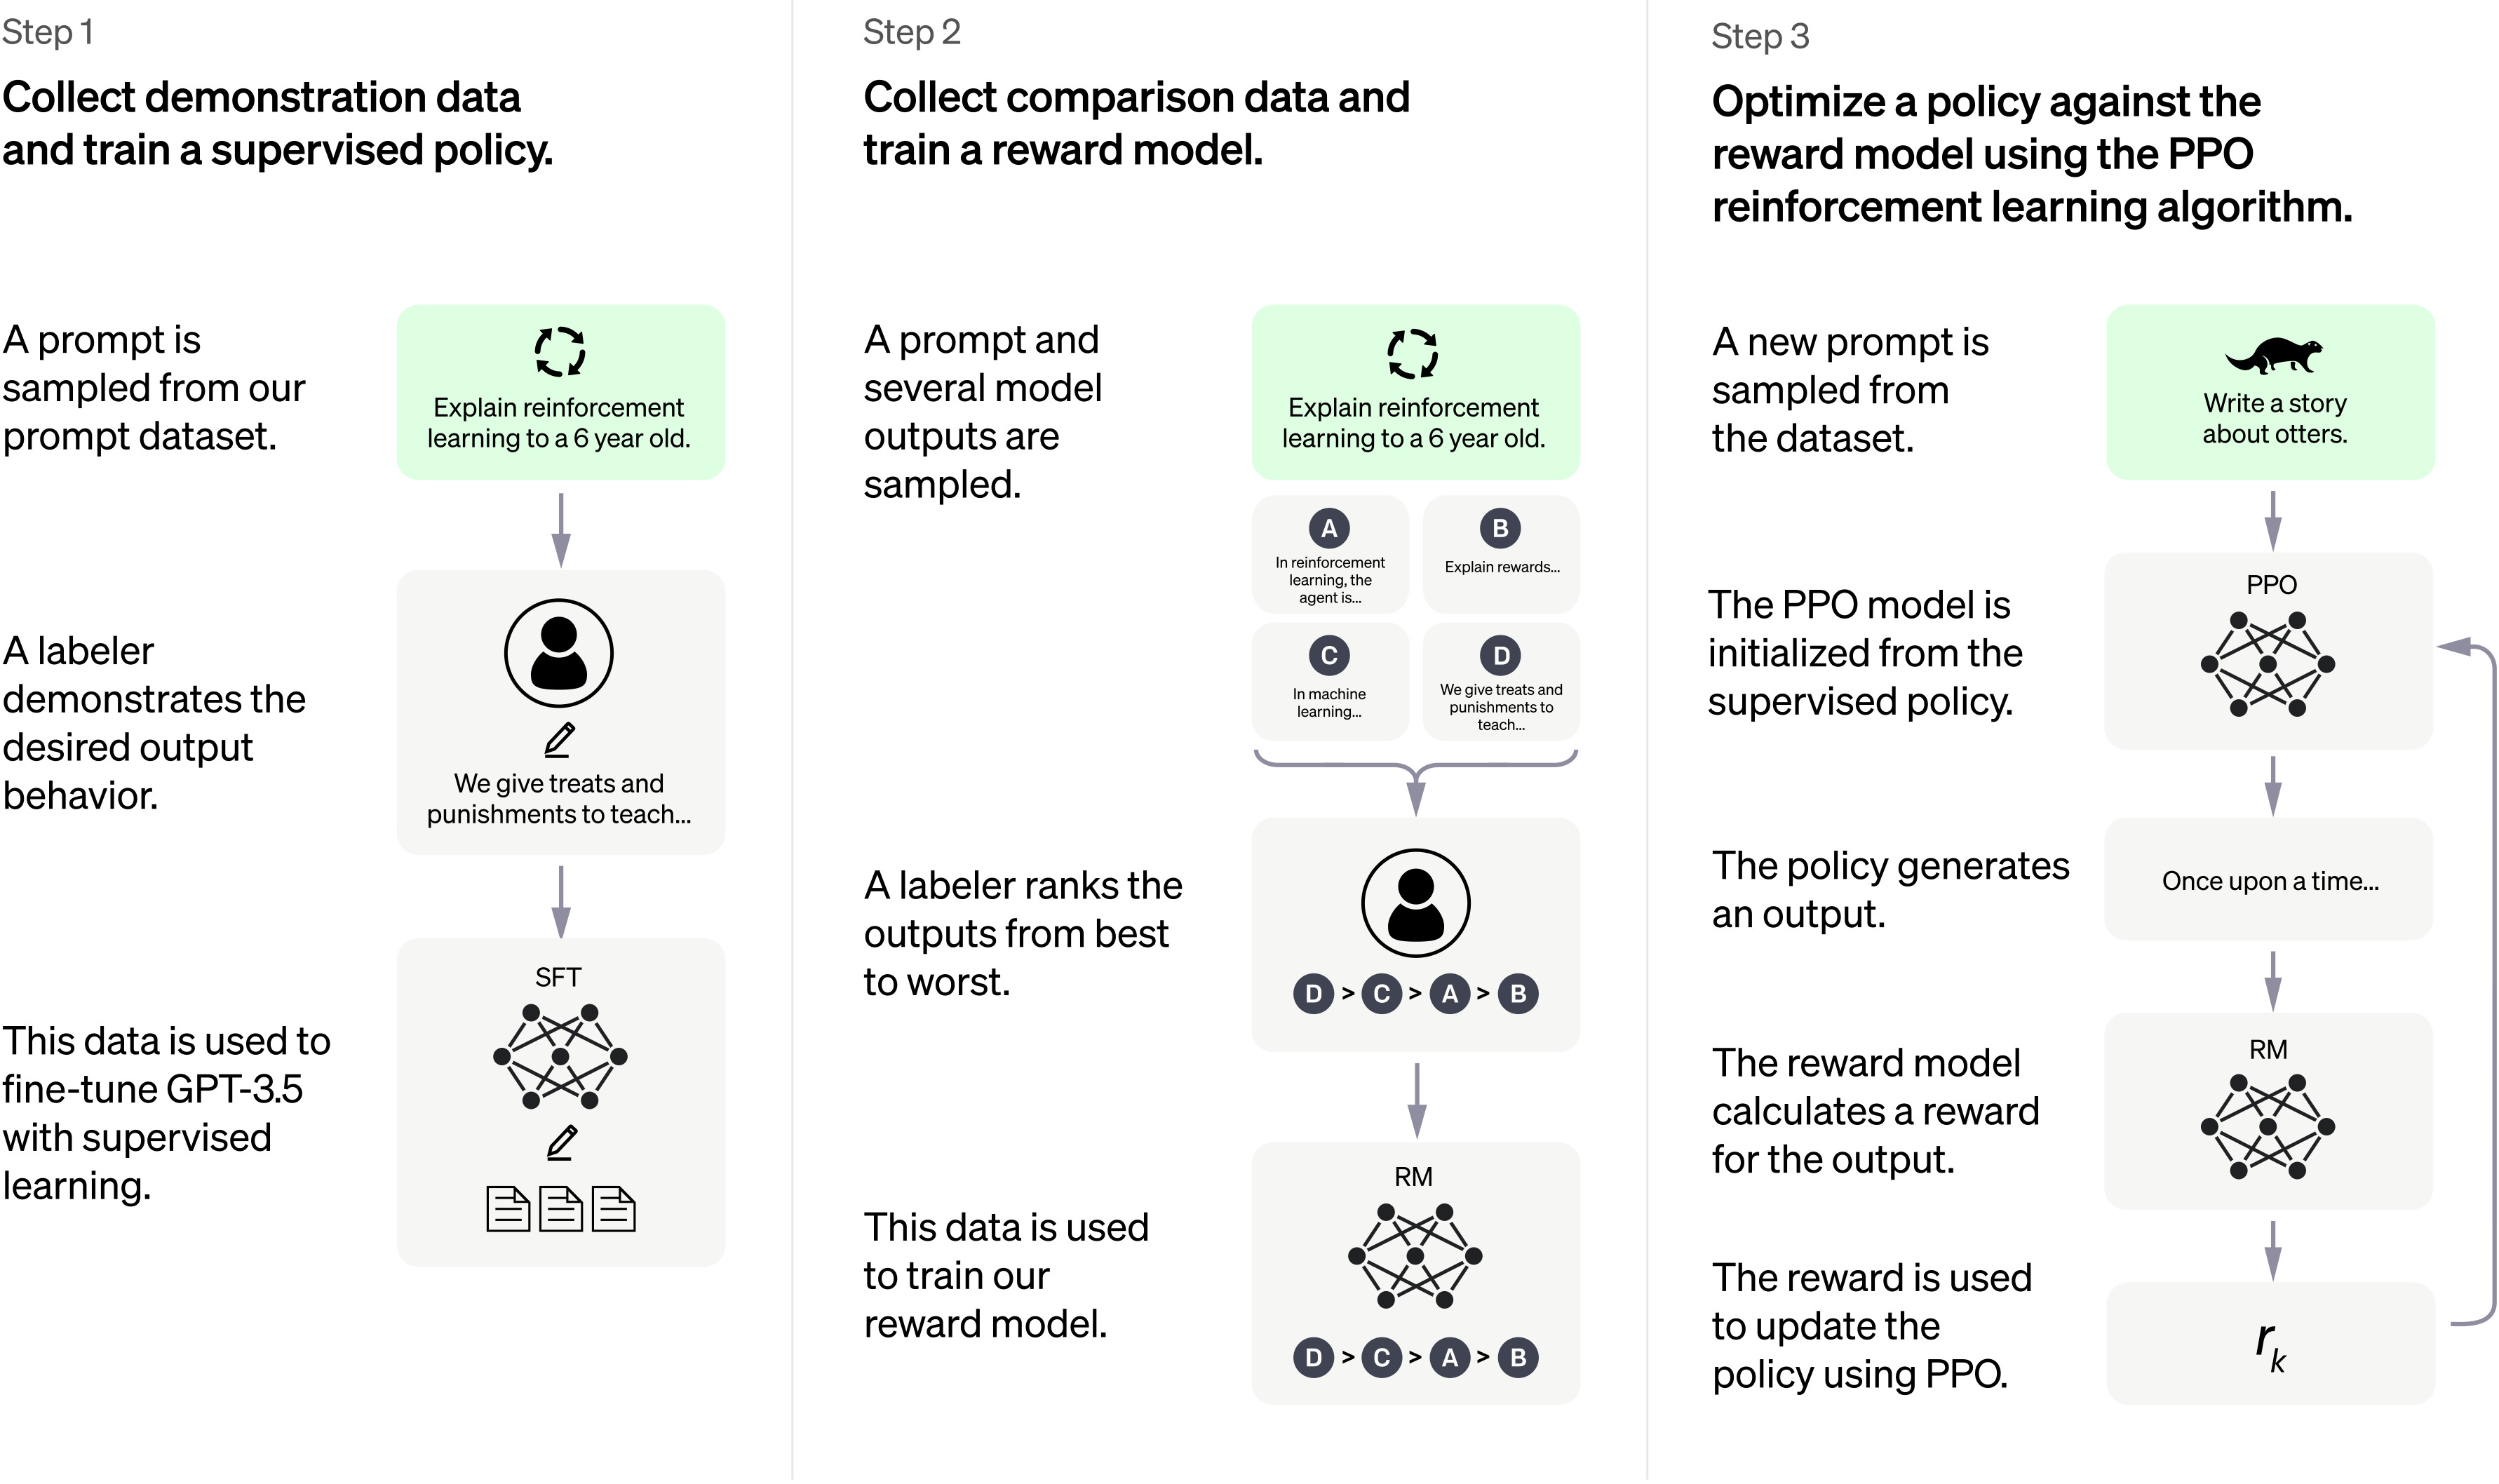
\includegraphics[scale=0.4]{ChatGPT_Diagram.jpg}
    \caption{Diagrama del metodo de entrenamiento
    para ChatGPT \cite{ej-chatgpt}}
    \label{fig:chatgpt-diagrama}
\end{figure}

% \begin{figure}
%     \centering
%     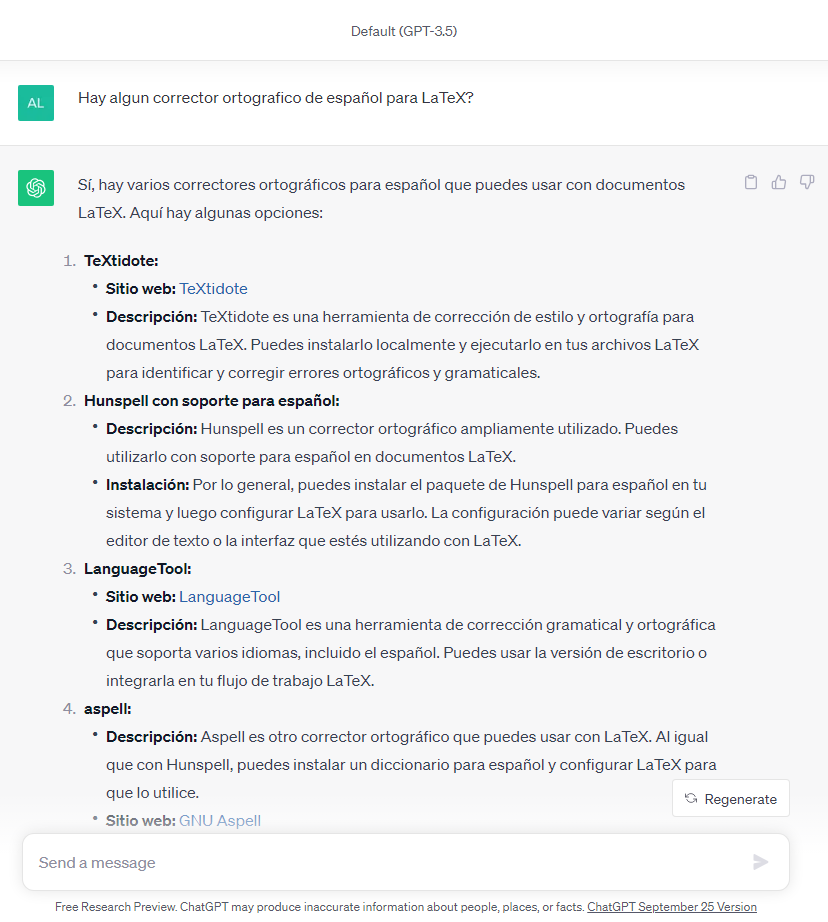
\includegraphics[scale=0.55]{ej1-chatgpt.png}
%     \caption{Ejemplo de consulta sobre corrector ortografico de español
%     para LaTeX}
%     \label{fig:chatgpt-ej1}
% \end{figure}

% \begin{figure}
%     \centering
%     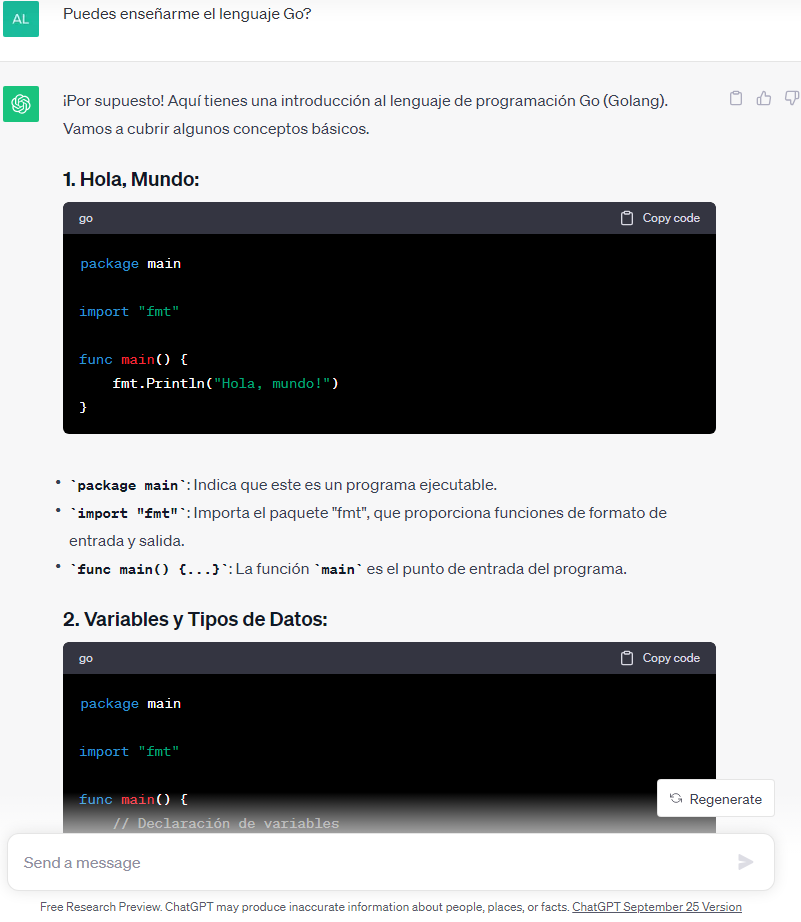
\includegraphics[scale=0.55]{ej2-chatgpt.png}
%     \caption{Ejemplo de consulta donde se le pide que enseñe el 
%     lenguaje de programacion Go}
%     \label{fig:chatgpt-ej2}
% \end{figure}

\newpage
\subsection{DALL-E}
De los mismos creadores de ChatGPT (OpenAI) DALL-E es otro caso de exito que muy
probablemente el lector ya lo conozca. Se trata  de una de las AI que comenzaron
esta revolucion de generar imagenes, junto a otras como \textit{Stable Diffusion}
y \textit{MidJourney}. \cite{dalle-xtaka}

DALL-E es un sistema de AI que tiene la capacidad de crear imagenes realistas y arte
dada una descripcion en lenguaje natural. ya que ha sido entrenada para distinguir 
las fórmulas que utilizamos al expresarnos y querer pedir o preguntar algo. \cite{ej-dalle}

Además de esto, DALL-E ha sido entrenada también mediante una gigantesca 
biblioteca de obras de arte y fotografías. Gracias a esto, 
cuando le pides que dibuje a una celebridad, DALL-E sabrá a quién te refieres, 
y dibujará el aspecto que tiene esta persona realizando una acción que también 
sabrá interpretar y dibujar. \cite{dalle-xtaka}

Además de esto, este sistema de inteligencia artificial es también capaz de combinar
conceptos, estilos y atributos para una imagen. 

\subsubsection{¿Como funciona?}
DALL-E fue creada al entrenar una red neuronal con imagenes y su descripcion en lenguaje
natural, a traves del DL no solo comprende objetos individuales sino que tambien aprende 
de las relaciones entre objetos. \cite{ej-dalle}

DALL-E utiliza lo que se llama un modelo de difusión, que son esos sistemas 
de inteligencia artificial capaces de crear imágenes de la nada. 
En este proceso de creación, aprende de las estructuras latentes de los datos 
para entrenarse para eliminar el ruido gaussiano de imágenes borrosas, 
que son esas pequeñas distorsiones que pueden generarse en este tipo de AI. 
\cite{dalle-xtaka}

Su proceso de creación se puede resumir en tres pasos. 
Primero, codifica y entiende el texto que le has escrito en el prompt 
distingue los diferentes rasgos, características y estilos que has pedido que dibuje.
Luego, DALL-E crea información de imagen a partir de esta petición, y finalmente 
utiliza un decodificador que pinta la imagen partiendo de ese texto. \cite{dalle-xtaka}

Aqui van unos ejemplos de lo que se puede hacer con DALL-E:

\begin{figure}
    \centering
    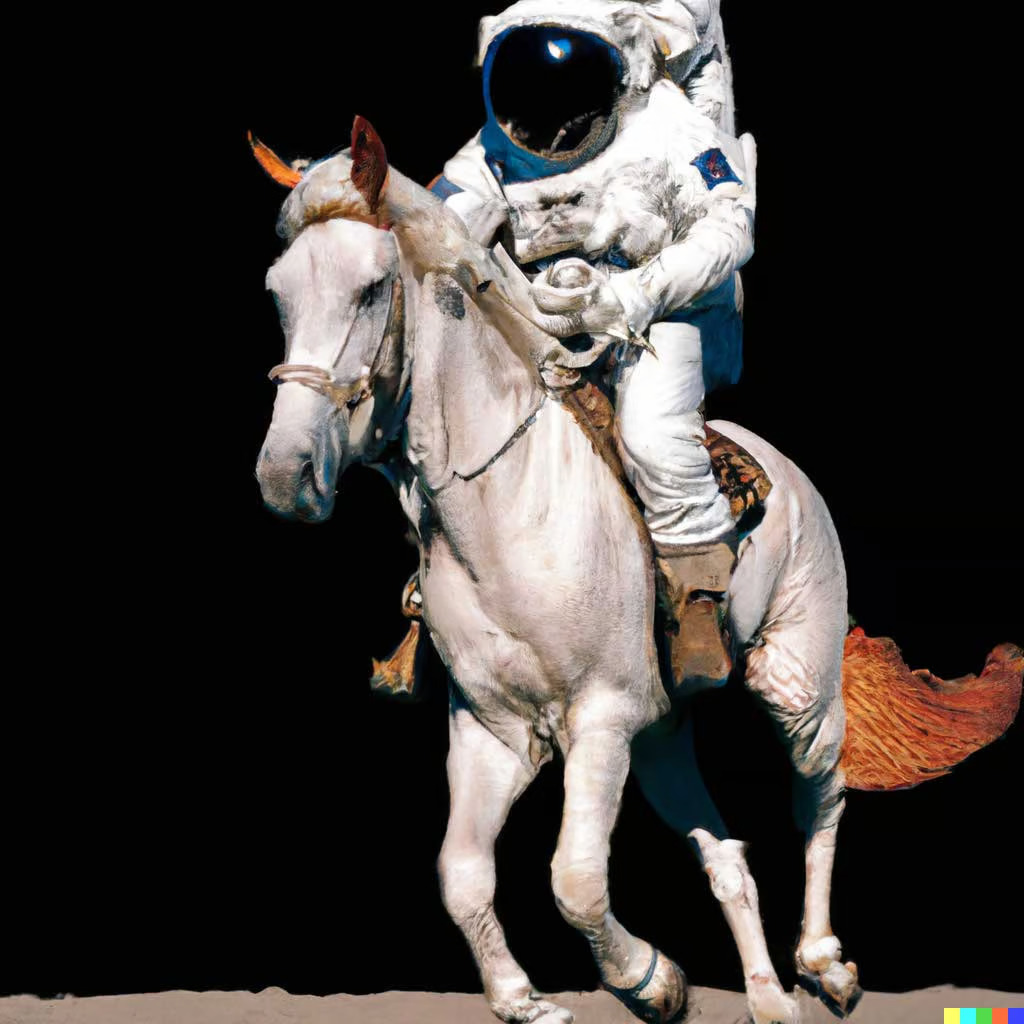
\includegraphics[scale=0.19]{ej1-dalle.jpg}
    \caption{Ejemplo de generacion de imagen: un astronauta montando un
    caballo con estilo fotorealistico \cite{ej-dalle}}
    \label{fig:dalle-ej1}
\end{figure}

\begin{figure}
    \centering
    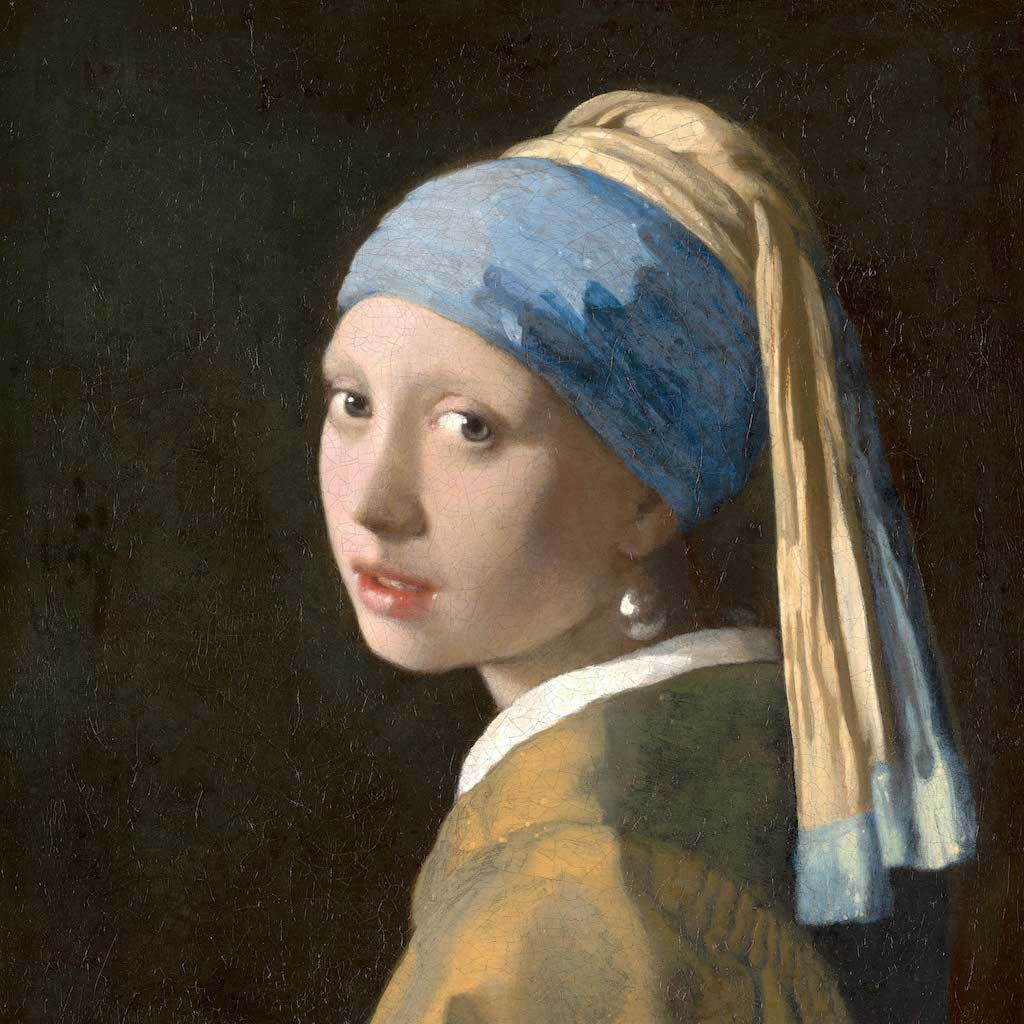
\includegraphics[scale=0.1]{ej2.1-dalle.jpg}
    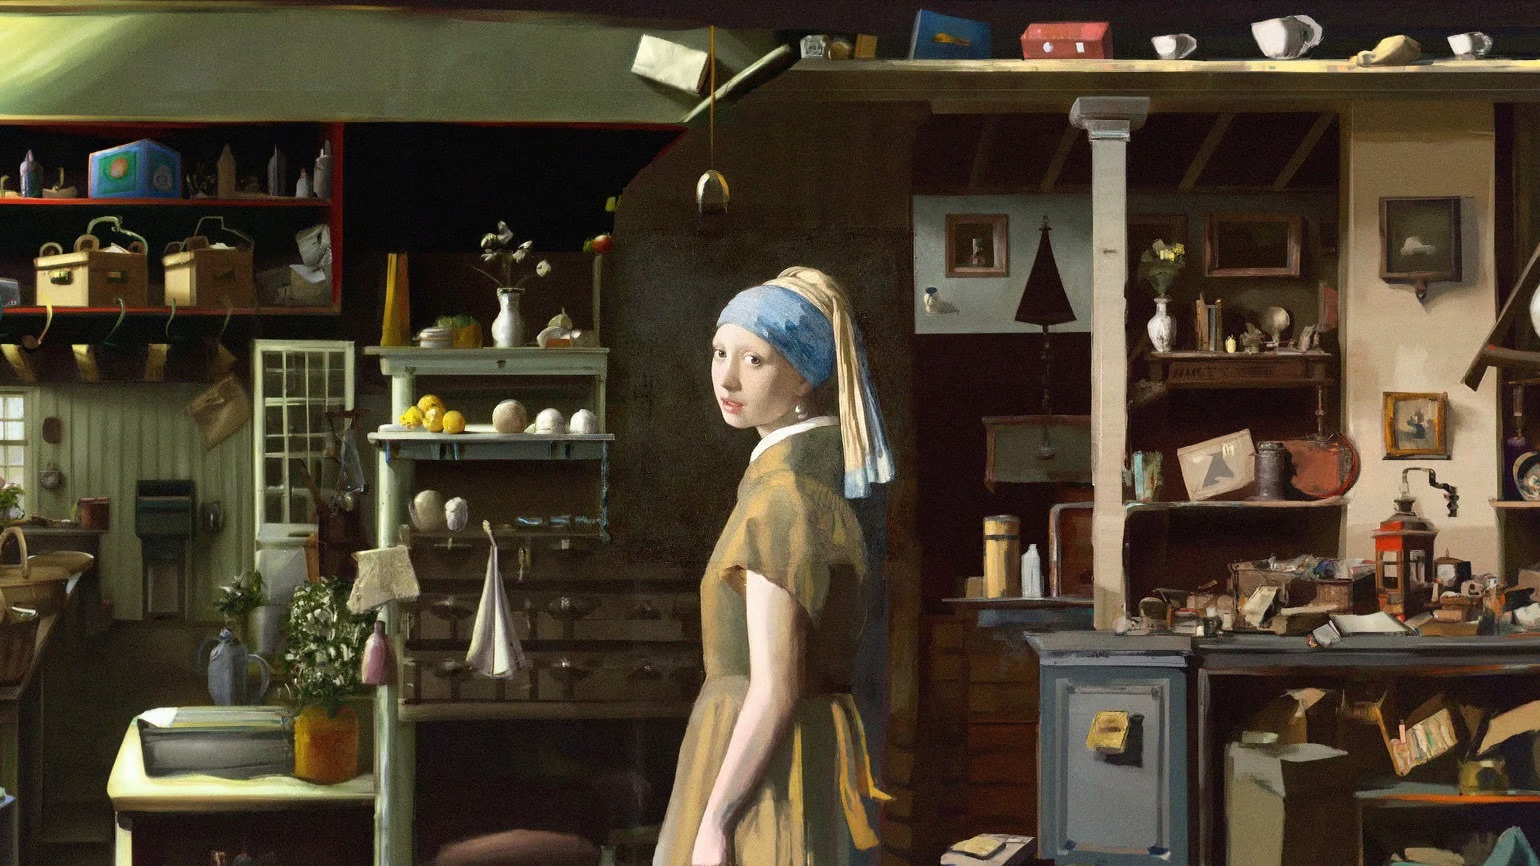
\includegraphics[scale=0.1182]{ej2.2-dalle.jpg}
    \caption{Ejemplo de \textit{Outpainting}: agregar contexto a una
    imagen \cite{ej-dalle}}
    \label{fig:dalle-ej2}
\end{figure}

\begin{figure}
    \centering
    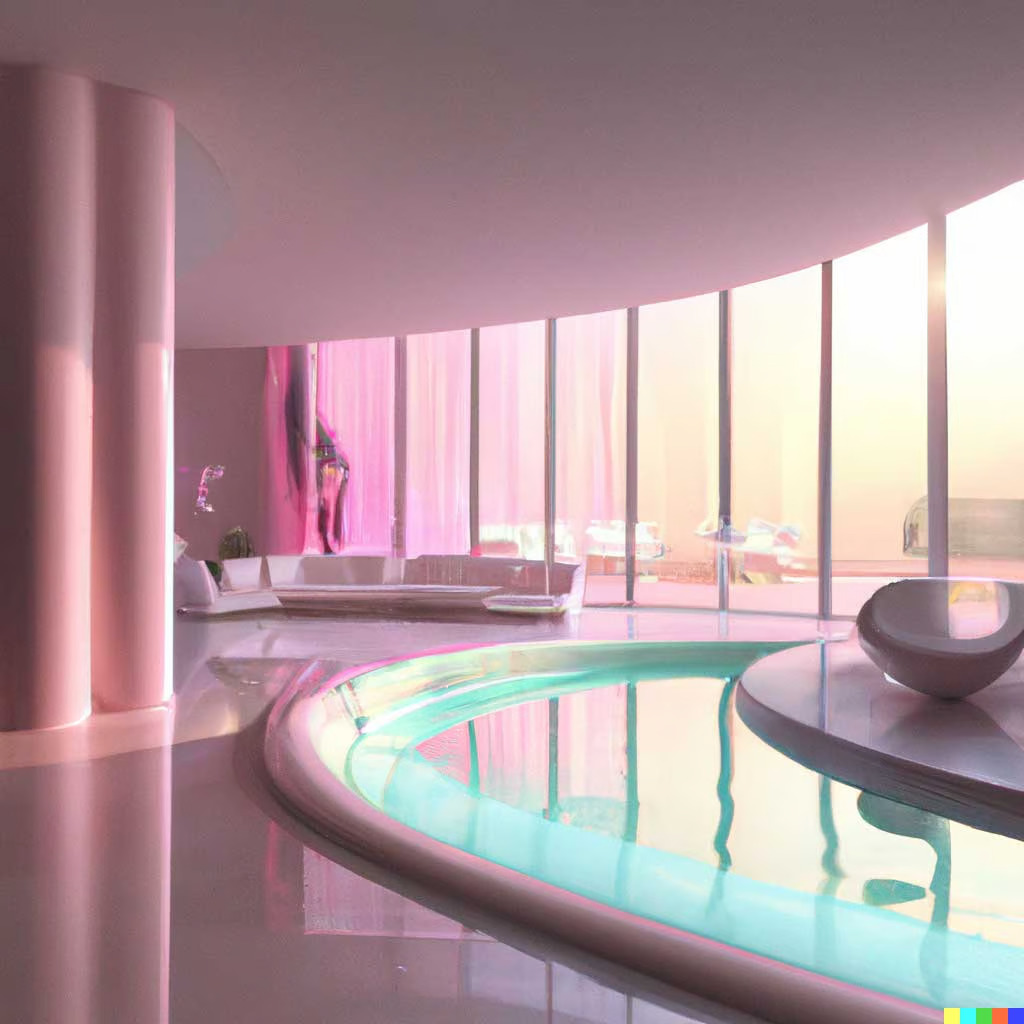
\includegraphics[scale=0.15]{ej3.1-dalle.jpg}
    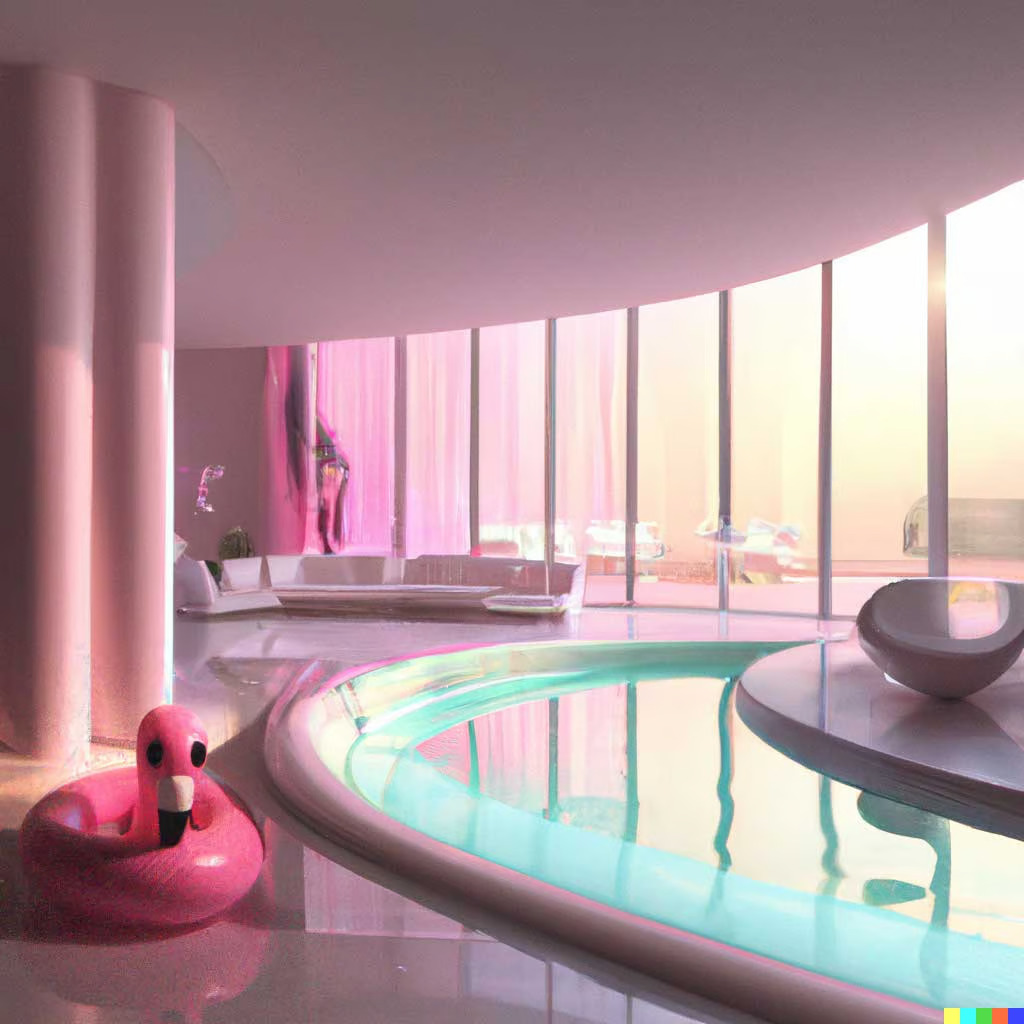
\includegraphics[scale=0.15]{ej3.2-dalle.jpg}
    \caption{Ejemplo de \textit{Inpainting} entrada: agrega un flamenco
    al lado de la piscina \cite{ej-dalle}}
    \label{fig:dalle-ej3}
\end{figure}

\begin{figure}
    \centering
    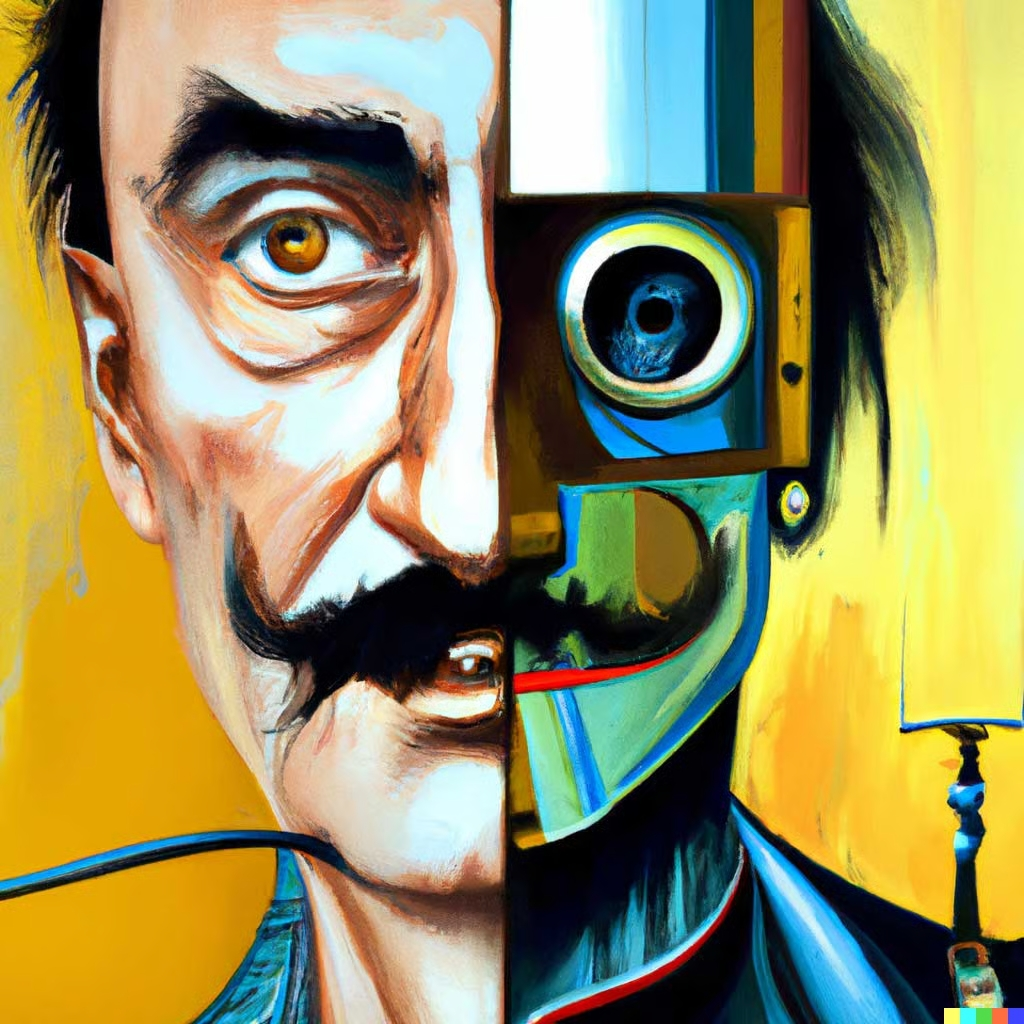
\includegraphics[scale=0.15]{ej4.1-dalle_1.jpg}
    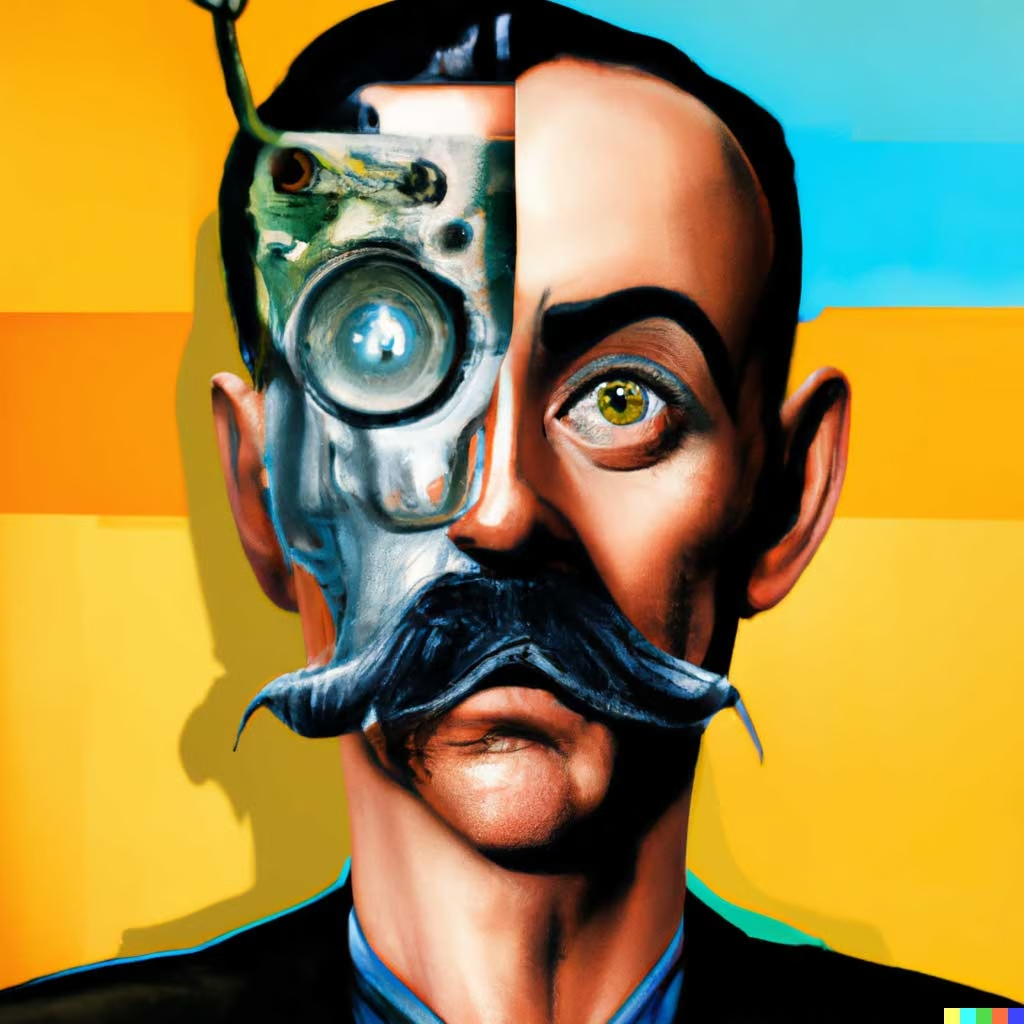
\includegraphics[scale=0.15]{ej4.2-dalle_1.jpg}
    \caption{Ejemplo de Variaciones de una imagen \cite{ej-dalle}}
    \label{fig:dalle-ej4}
\end{figure}
\newpage
\subsection{DeepFake}
La tecnologia \textit{deepfake} es una tecnica que manipula imagenes o videos por medio del 
\textit{deep learning}. El resultado es una imagen o video muy realista de un evento que nunca ocurrio.
\cite{ej-deepfake2}

Un \textit{deepfake} es una imagen o un vídeo falsificado digitalmente de una persona 
que la hace parecer otra persona. Es el siguiente nivel de creación de contenido falso 
que aprovecha la inteligencia artificial. \cite{ej-deepfake2}

La gente empezó a tomar conciencia de la tecnología deepfake cuando un usuario de Reddit 
llamado \textquotedblleft{}Deepfakes\textquotedblright{} publicó que había desarrollado
un algoritmo de ML que podía transponer rostros de celebridades sin problemas
a vídeos de contenido para adultos. \cite{ej-deepfake2}
 
\subsubsection{¿Como funciona?}
Un vídeo deepfake explota dos modelos de \textit{machine learning}. 
Un modelo crea falsificaciones a partir de un conjunto de datos de vídeos de muestra, 
mientras que el otro intenta detectar si el vídeo es realmente un fraude. 
Cuando el segundo modelo ya no puede decir si el vídeo es falso, 
el deepfake probablemente también sea lo suficientemente creíble para un 
espectador humano. 
Esta técnica se llama
\textquotedblleft{}red generativa adversarial\textquotedblright{} (GAN). \cite{ej-deepfake2}

\textquotedblleft{}Un modelo generativo G que captura la distribución de los datos, 
y un modelo discriminativo D que estima la probabilidad de que una muestra 
provenga de los datos de entrenamiento y no de G. 
El procedimiento de entrenamiento de G es maximizar la probabilidad de que D se equivoque.
\textquotedblright{}
\cite{ej-deepfake4}


Los GAN son una tecnología pionera en el campo de la visualización por computadora 
y tienen mucho éxito a la hora de generar imágenes que se parecen a las humanas.
El principal reto de la tecnología solía ser la disponibilidad de datos de entrenamiento 
para una persona determinada. Por eso, al disponer de muchos datos, 
los deepfakes de famosos fueron muy populares al principio.

\subsubsection{Tipos de deepfake}
Hay tres tipos principales de tecnología deepfake \cite{ej-deepfake2}
\begin{itemize}
    \item{\textbf{Deepfakes con intercambio de rostros:} este es el tipo más común de deepfake 
    que implica intercambiar el rostro de una persona con el de otra en un video o una imagen.}
    \item{\textbf{Deepfakes de audio:} reemplazan la voz de alguien en una grabación por 
    la de otra persona.}
    \item{\textbf{Deepfakes textuales:} generan texto que parece haber sido escrito 
    por otra persona.}
\end{itemize}
Aqui van unos ejemplos:
\begin{figure}
    \centering
    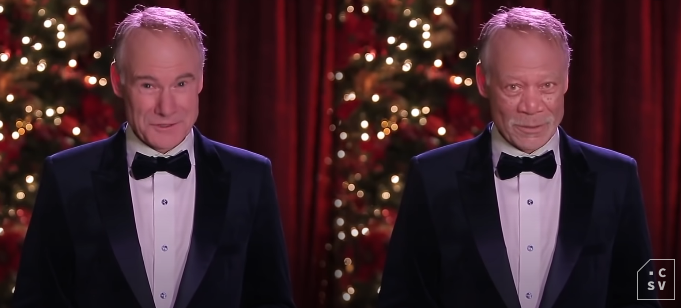
\includegraphics[scale=0.55]{ej1-deepfake.png}
    \caption{Ejemplo de intercambio de rostros \cite{ej-deepfake3}}
    \label{fig:deepfake-ej1}
\end{figure}

\begin{figure}
    \centering
    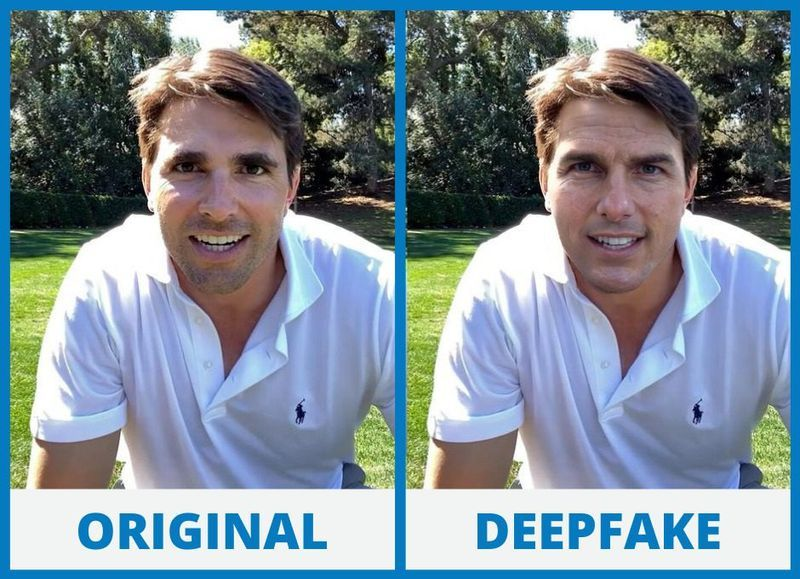
\includegraphics[scale=0.3]{ej3-deepfake.jpeg}
    \caption{Ejemplo de intercambio de rostros \cite{img-deepfake}}
    \label{fig:deepfake-ej3}
\end{figure}

\begin{figure}
    \centering
    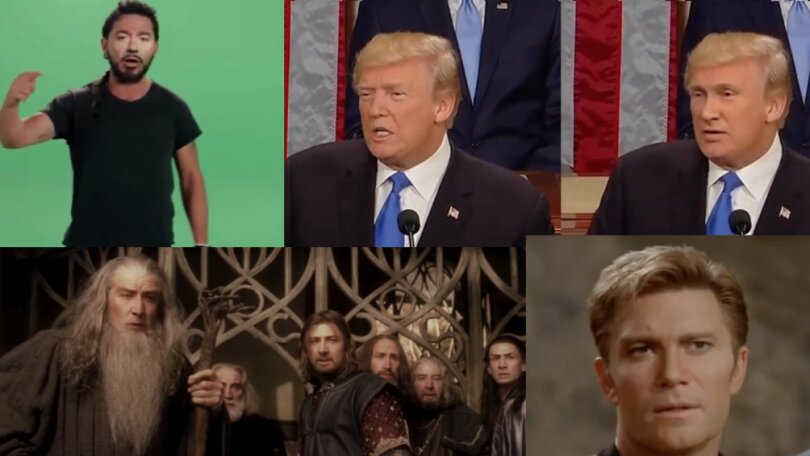
\includegraphics[scale=0.35]{ej4-deepfake.jpg}
    \caption{Ejemplo de intercambio de rostros \cite{ej-deepfake1}}
    \label{fig:deepfake-ej4}
\end{figure}

\newpage
\subsection{Nvidia DLSS}
DLSS (\textit{Deep Learning SuperSampling}) Es un tipo de técnica de 
renderizado de video que busca aumentar la velocidad de cuadros por
segundo, renderizando cuadros a una resolución más baja que la mostrada.

El \textit{SuperSampling} hace
referencia a un metodo \textit{anti-aliasing} que suaviza los bordes 
irregulares que aparecen en los gráficos renderizados. 
Sin embargo, a diferencia de otras formas de anti-aliasing, 
SSAA (\textit{supersampling anti-aliasing}) funciona renderizando la imagen 
a una resolución mucho más alta y usando esos datos para llenar 
los espacios en la resolución nativa. \cite{ej-dlss}

DLSS es el resultado de un proceso exhaustivo de enseñanza del algoritmo
de inteligencia artificial de Nvidia para generar juegos más atractivos.
Después de renderizar el juego a una resolución más baja, 
DLSS infiere información de su base de conocimientos de entrenamiento 
de imágenes de superresolución para generar una imagen que todavía 
parece estar ejecutándose a una resolución más alta. 
La idea es hacer que los juegos renderizados a 1440p parezcan 
ejecutarse en 4K o que los juegos a 1080p parezcan 1440p. \cite{ej-dlss}

Es necesario aclarar que para utilizar el DLSS necesitamos hardware específico
de nvidia, las graficas RTX series 2000 (para DLSS1) series 3000 (para DLSS2)
series 4000 (para DLSS3)

El exito de DLSS hizo que AMD y luego Intel se apresuren en competir, con sus tecnologías
FSR y XeSS respectivamente.

\subsubsection{¿Como funciona?}
La NN recibe dos entradas: 
\begin{itemize}
    \item{Imagenes aliased de baja resolucion generadas por el motor del
    juego}
    \item{En baja resolucion, vectores de movimiento de las mismas imagenes,
    tambien generados por el motor del juego.}
\end{itemize}

\begin{figure}
    \centering
    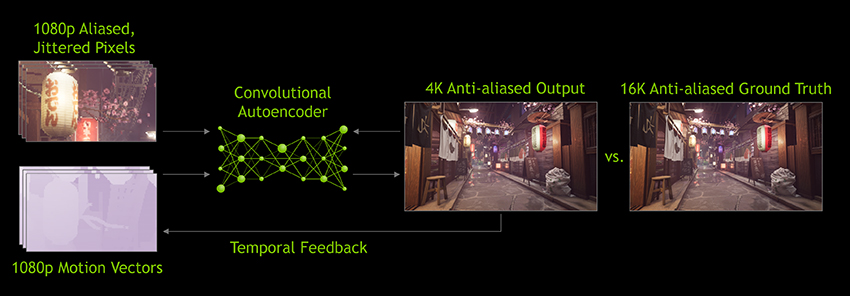
\includegraphics[scale=0.4]{dlss.jpg}
    \caption{Arquitectura de Nvidia DLSS 2.0 \cite{ej-dlss2}}
    \label{fig:arquitectura-dlss}
\end{figure}

En este enfoque, los vectores de movimiento sirven para indicar la dirección 
en la que los objetos de una escena se desplazan de un cuadro a otro. 
Estos vectores se aplican nuevamente a la salida de alta resolución 
del cuadro anterior para prever cómo se visualizará en el próximo cuadro. 
Este procedimiento se denomina 
\textquotedblleft{}Retroalimentación Temporal\textquotedblright{}
porque utiliza la información pasada para anticipar eventos futuros. 
En el transcurso del aprendizaje, la imagen generada se compara con una 
imagen pre-renderizada de alta calidad con resolución de 16k.
Las discrepancias entre estas dos imágenes se retroalimentan a la red neuronal 
para perfeccionar y optimizar sus resultados. \cite{ej-dlss2}

Este ciclo se repite innumerables veces en una supercomputadora de Nvidia. 
Una vez que el modelo produce imágenes de calidad satisfactoria, 
se distribuye a los usuarios a través de actualizaciones de controladores 
para sus tarjetas gráficas. \cite{ej-dlss2}

En pocas palabras podemos decir que es un proceso iterativo de entrenamiento, 
donde la historia de las imágenes y la retroalimentación constante impulsan 
la mejora continua del modelo, que luego se implementa en las tarjetas gráficas 
de los usuarios mediante actualizaciones de controladores. 

A continuacion van ejemplos que muestran el impacto de dlss3 en los fps.

\begin{figure}
    \centering
    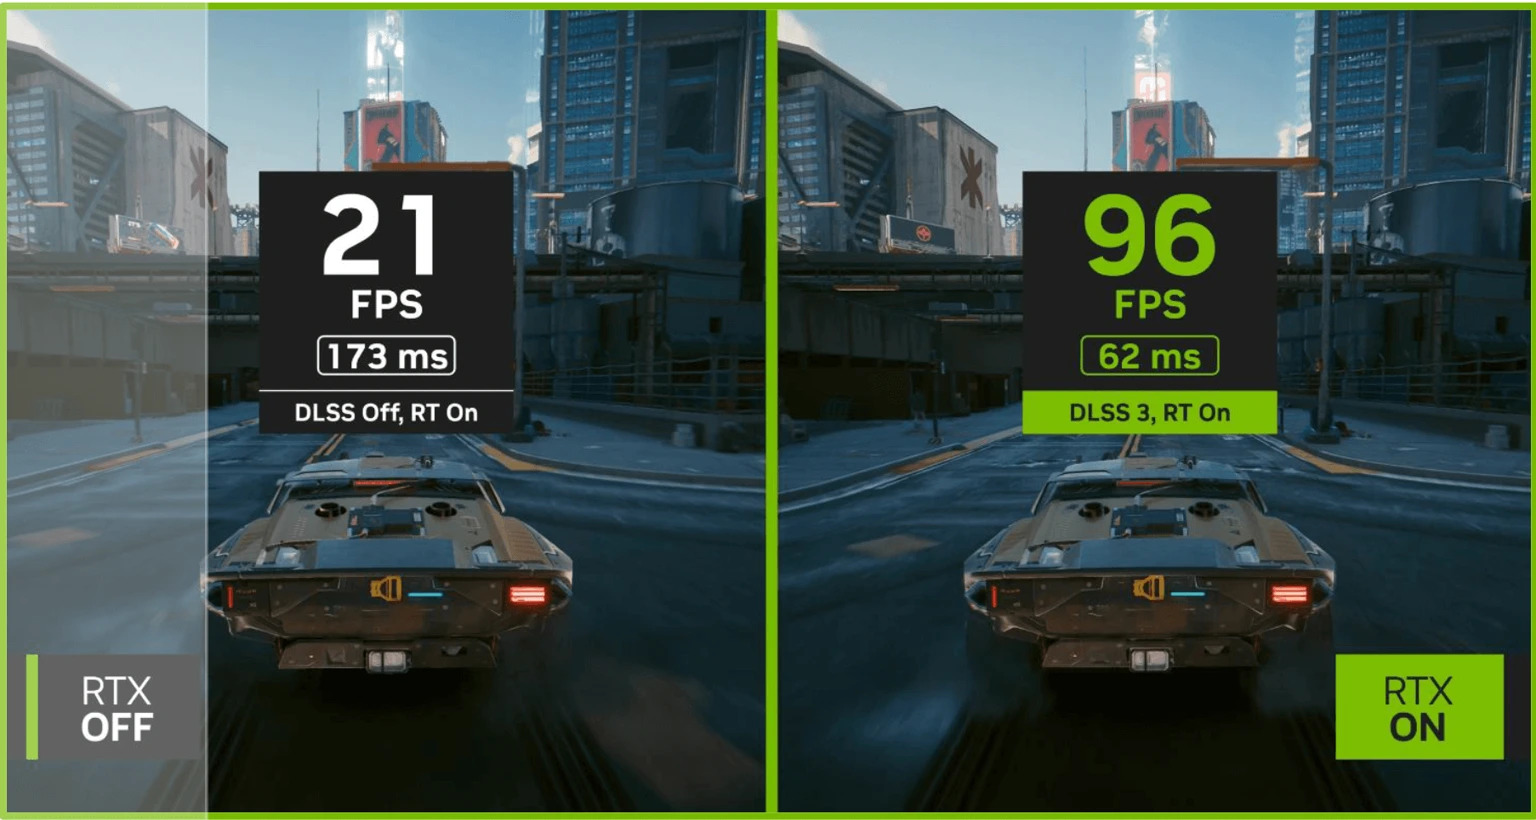
\includegraphics[scale=0.15]{ej1-dlss3.jpg}
    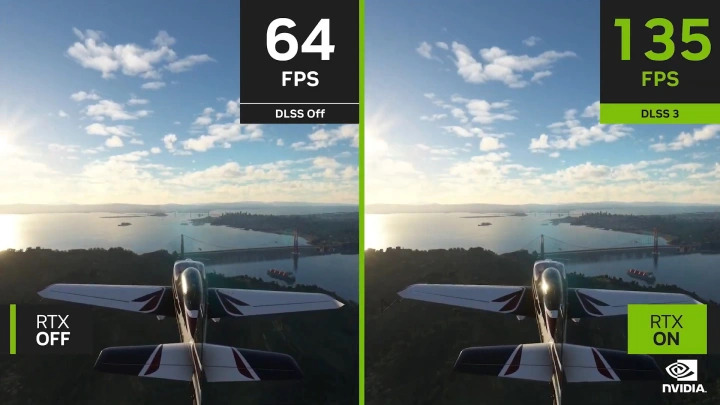
\includegraphics[scale=0.32]{ej2-dlss3.jpg}
    \caption{Impacto de DLSS3 en los juegos Cyberpunk 2077 y 
    Microsoft flight simulator \cite{img1-dlss3}}
    \label{fig:ej1-dlss3}
\end{figure}
\newpage

\subsection{SAM}
La segmentación de imágenes es un método que divide una imagen digital 
en subgrupos (segmentos) para reducir la complejidad de esta y, así, 
poder facilitar su procesamiento o análisis. La finalidad de la segmentación 
es asignar etiquetas a píxeles para identificar objetos, personas u otros 
elementos en la imagen. 

La segmentación de las imágenes es clave para las tecnologías y 
algoritmos de visión artificial, pero también se utiliza hoy en día para 
muchas aplicaciones como, por ejemplo, el análisis de imágenes médicas, 
la visión de los vehículos autónomos, el reconocimiento y la detección de 
rostros o el análisis de imágenes satelitales, entre otras. \cite{ej3-SAM}

SAM (\textit{Segment Anything Model}) \textquotedblleft{}las tijeras mas
potentes de la Inteligencia artificial\textquotedblright{} es un modelo
\textit{open source} desarrollado por META.
Busca impulsar una idea muy potente en el mundo de \textit{computer vision} asi
como los modelos GPT revolucionaron el mundo del procesamiento del lenguaje natural.
\cite{ej-SAM}

El punto fuerte de SAM esta en el \textit{anything} aqui es su diferencia con otros
modelos de segmentacion donde de antemano el modelo ya sabe que segmentar (como
un problema de aprendizaje supervisado) SAM es capaz de generalizar la nocion de
objeto, es capaz de desplegar sus habilidades en contextos que nunca a visto durante
su entrenamiento (\textit{zero-shot learning}) \cite{ej-SAM}

SAM es un modelo flexible que fue entrenado con el conjunto de datos más grande
hasta la fecha, llamado SA-1B y que cuenta con 11 millones de imágenes y 1.1 mil millones 
de máscaras en segmentación. Gracias a estos datos, SAM es capaz de detectar todo tipo de 
objetos sin necesidad de un entrenamiento adicional. \cite{ej3-SAM}

\begin{figure}
    \centering
    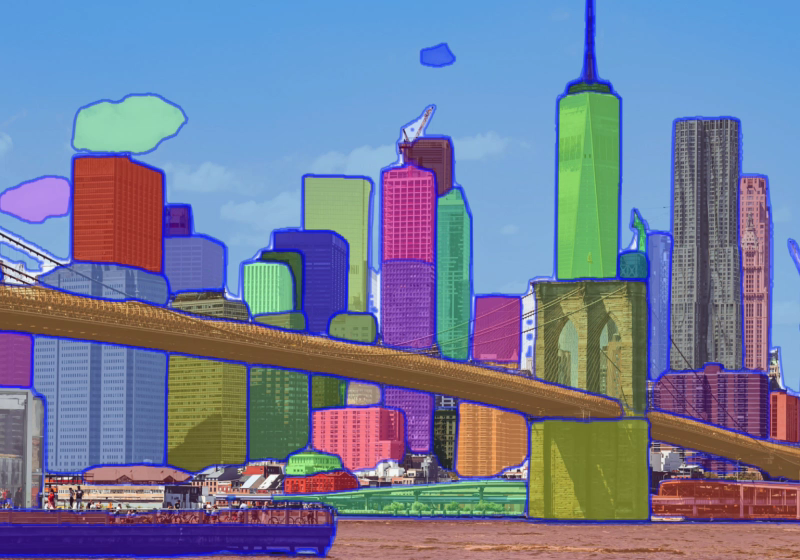
\includegraphics[scale=0.28]{ej1-SAM.png}
    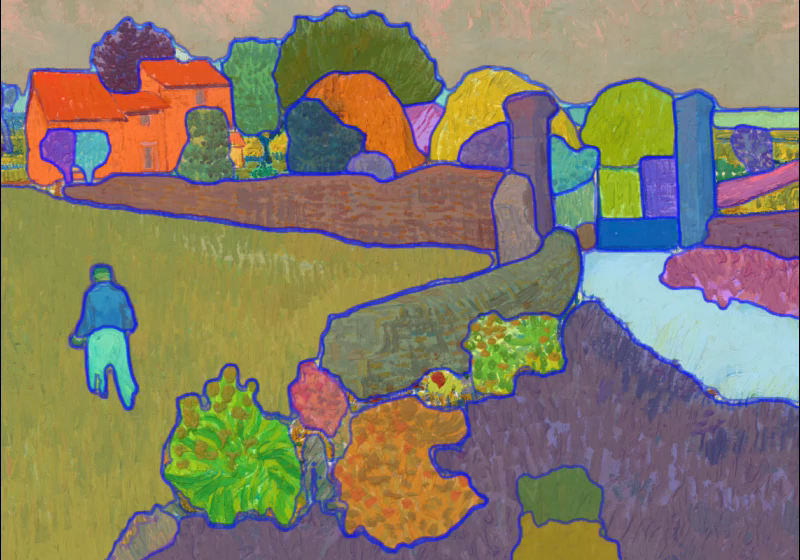
\includegraphics[scale=0.28]{ej2-SAM.png}
    \caption{Ejemplos de SAM \cite{ej-SAM}}
    \label{fig:ej-SAM}
\end{figure}

\subsection{Alphafold}
Es un sistema de inteligencia artificial desarrollado por DeepMind 
que predice la estructura 3D de una proteína a partir de su secuencia de aminoácidos. 
Regularmente logra una precisión competitiva con el experimento. 

DeepMind y el Instituto Europeo de Bioinformática (EMBL-EBI) del EMBL se han asociado 
para crear una base de datos \textit{AlphaFold DB} para que estas predicciones estén disponibles 
gratuitamente para la comunidad científica. 

La última versión de la base de datos contiene más de 200 millones de entradas, 
lo que proporciona una amplia cobertura de UniProt 
(el repositorio estándar de secuencias y anotaciones de proteínas). 
\cite{ej-alphafold}

El alcance de AlphaFold es enorme, hasta tal punto que Pushmeet Kohli, 
director de IA de DeepMind, considera que se trata de la 
\textquotedblleft{}mayor contribución de la IA al conocimiento científico hasta la fecha
\textquotedblright{}. \cite{ej-alphafold2}

Hasta ahora, entender la compleja estructura de cada proteína requería 
largos y tediosos experimentos para comprobar su forma final y poder diseñar 
medicamentos específicos. Ahora, ese trabajo lo realiza la IA con una precisión altísima.
La velocidad con la que la IA es capaz de entender la estructura de las proteínas 
es muchísimo más rápida de lo que los humanos podemos hacer manualmente. 
Para equiparar el trabajo de AlphaFold, los humanos sin esta tecnología habríamos 
tardado miles de años. \cite{ej-alphafold2}

\textquotedblleft{}Determinar la estructura 3D de una proteína solía tardar muchos meses o años, 
ahora toma segundos. Con esta nueva adición de estructuras que describen casi 
todo el universo de proteínas, podemos esperar que se resuelvan más misterios 
biológicos cada día\textquotedblright{}, ha descrito Eric Topol, director del Scripps Research, 
uno de los centros biomédicos más prestigiosos del mundo. \cite{ej-alphafold2}


\begin{figure}
    \centering
    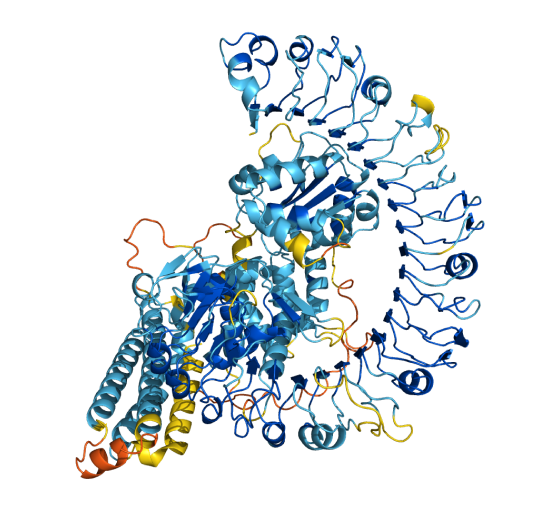
\includegraphics[scale=0.4]{ej1-alphafold}
    \caption{Q8W3K0: Una proteína potencial de resistencia a enfermedades de las plantas. 
    PLDDT medio 82,24. \cite{ej-alphafold}}
    \label{fig:ej-alphafold}
\end{figure}

\newpage
\section{Conclusion}
Es evidente que las redes neuronales son una herramienta poderosa, se destaca 
la prominente influencia de estas herramientas en diversos campos. 
Desde la capacidad para aprender patrones complejos  hasta su aplicación en áreas 
como visión por computadora, procesamiento de lenguaje natural, medicina, etc.
Queda en evidencia su versatilidad y potencial transformador.

El continuo avance en la investigación y desarrollo promete aún más innovaciones y 
descubrimientos en el futuro. Estos avances no solo mejorarán la eficiencia y precisión 
de las aplicaciones existentes, sino que también abrirán nuevas oportunidades 
en áreas emergentes.

% =================================================================================
% Bibliografia
% =================================================================================
\printbibliography

\end{document}